\section{Функционална част}
    \subsection{Сигурност}
    За осъществяване на сигурността е използван Spring Security, което позволява защитаването на крайните точки на API-то, в този случай, с Basic Auth. Spring Security действа като филтър, който се изпълнява върху крайните точки, които са опоменати като нуждаещи се от защита. Тези точки са:
    \begin{itemize}
        \item ``/application/**''
        \item ``/task/**''
        \item ``/work/**''
        \item ``/review/**''
        \item Всички действия върху ``/user/**'' освен ``/user/login'' и POST ``/user''
    \end{itemize}
    
    За да се конфигурира защитата на крайните точки, се създава клас, който да разширява класа WebSecurityConfigurerAdapter и да имплементира два метода, обозначаващи крайните точки, които да бъдат защитени и клас, дефиниращ извличането на информацията за потребител от базата данни.
 
    \begin{figure}[h]
        \centering
        \makebox[\textwidth][c]{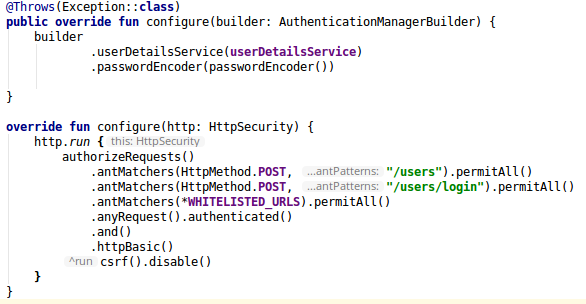
\includegraphics[width=1\textwidth]{images/securityMethods.png}}%
        \caption{}
        \label{fig:security_methods}
    \end{figure}

    Във фигура \ref{fig:security_methods} са дефинирани крайните точки, които да бъдат защитени. ``WHITELISTED\textunderscore URLS'' e списък от крайни точки, които не изискват защита, а чрез ``anyRequest().authenticated()'' определяме всяка останала крайна точка да изисква защита. 
    В първия метод на фигура \ref{fig:security_methods} userDetailsService е обект от тип PostgreUserDetailsService, който дефинира извличането на данните от базата и проверката на правата на конкретния потребител. Имплементацията му е показана във фигура \ref{fig:user_details_service}
    
     \begin{figure}[h]
        \centering
        \makebox[\textwidth][c]{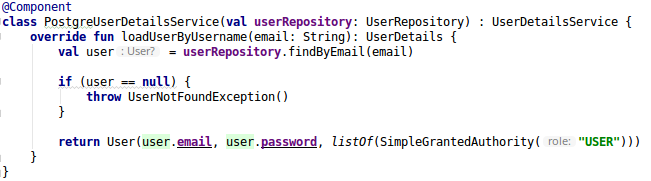
\includegraphics[width=1\textwidth]{images/userDetailsService.png}}%
        \caption{}
        \label{fig:user_details_service}
    \end{figure}
    
    
    
    \subsection{Модели}
    Моделите са начин за изобразяване на таблиците в базите данни чрез абстракции. Това се случва чрез създаване на клас, анотиран с ``Entity'', предоставна от Spring Data JPA. Класът трябва да има полета, представляващи колона от таблицата, с която искаме да работим. 
    Пр. Класът User трябва да има поле ``firstName''. По този начин при запазване на обекта в хранилището ще се добави нов ред в таблицата ``User'' с попълнените полета. В проекта има шест такива модела.
    Всеки модел удължава клас на име ``BaseEntity'', който съдържа полета ``Id'', ``createdAt'' и ``updatedAt'', както е показано на фигура \ref{fig:base_entityl}
    
    \begin{figure}
        \centering
         \makebox[\textwidth][c]{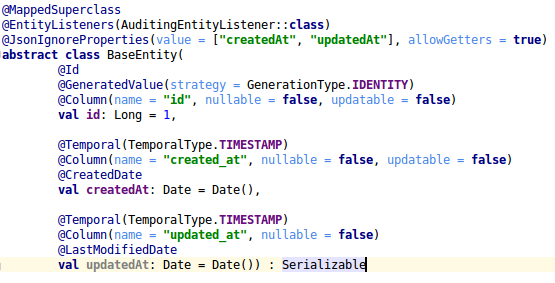
\includegraphics[width=1\textwidth]{images/base_entity.png}}%
        \caption{BaseEntity}
        \label{fig:base_entityl}
    \end{figure}
    
    Чрез анотацията ``@MappedSuperclass''' дефинираме класа ``BaseEntity'' като супер клас, на който полетата биват наследени от останалите модели. Тоест полетата, които съществуват в него като ``Id'' ще бъдат наследени и от останалите модели.
    
    ``@JsonIgnoreProperties'' казва на Spring да не десериализира подадените полета. Целта на това е да не се връщат стойностите им, тъй като няма нужда да се използват от клиентите. Съществуването на тези полета е единствено за удобството на бек енд-а.
    
    Във всяка таблица трябва да съществува първичен ключ, който уникално да идентифицира всеки ред от таблицата. Това се случва чрез анотацията ``Id'', която оказва полете, над което е поставено като първичен ключ. Освен това искаме уникалния идентификатор да бъде атоматично генериран при вмъкването на нов ред в таблицата. Това се случва чрез анотацията ``GeneratedValue'', което подавайки му типа на генериране като ``Identity'' добавя нов ред с уникален, генериран идентификатор. 
    Чрез анотацията ``Column'' можем да променяме параметри за съответната колона. В контекста на класа е използва за преименуването на колоната.
    
    Всеки следващ модел в документацията ще наследява този клас, тоест ще има тези полета в таблицата си.
    
        \subsubsection{User модел}
        User модела представлява абстракцията на User таблицата в PostgreSQL базата данни. 
        Таблицата притежава следните полета:
        \begin{itemize}
            \item firstName - Първото име на потребителя
            \item lastName - Фамилията на потребителя
            \item email - Електронният мейл на потребителя
            \item password - Паролата на потребителя
            \item dateOfBirth - Датата на раждане на потребителя
            \item phoneNum - Мобилният телефон на потребителя
        \end{itemize}
        
        \begin{figure}[h]
            \centering
            \makebox[\textwidth][c]{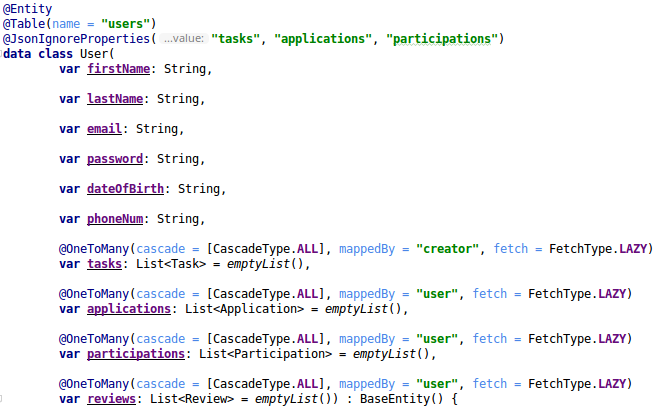
\includegraphics[width=1\textwidth]{images/user_entity.png}}%
            \caption{}
            \label{fig:user_entity}
        \end{figure}
        
        Чрез анотацията ``Table'' използвана във фигура \ref{fig:user_entity} специфично казваме как желаем таблицата да бъде именувана. Ако не предоставим тази информация Spring Data ще кръсти таблицата спрямо името на класа. Важна роля в класа играят полетата анотирани с ``OneToMany''. Това е една от анотациите предоставени от Spring Data, която дефинира връзката между класа и типа на полетата, върху който е поставен. User таблицата има връзка ``OneToMany'' с таблицата Таск. Това означава, че множество редове от типа Task могат да принадлежат на един User, но един Task може да бъде притежаван от само един User. Тези полета обаче няма да бъдат добавени като стойности в таблицата User. Те съществуват единствено за улеснение на програмиста. При желание да извлечем всички Task-ове, които принадлежат на конкретен User, Spring Data автоматично ще извлече и създадените от него съответни Task-ове.
        В анотацията можем също да изберем какво да се случва със създадените от потребител ресурси при неговото манипулиране. Това се случва чрез дефинирата на ``CascadeType.ALL''. Това ще извърши всички действия, които се извършват върху потребител и върху неговите Task-ове. Примерно при изтриване на User ще бъдат изтрите и неговите Task-ове, които е създал. 
        Тъй като е възможно един ред от таблица да притежава голям брой редове от друга таблица може да е неефикасно да се извличат всеки път ресурсите, които са създаден от него. Поради тази причина можем специфично да кажем на Spring Data как желаем данните да бъдат извличани. Имаме избор между ``FetchType.LAZY'' и ``FetchType.EAGER''. При първият начин данните ще бъдат извлечени единствено когато се извика Get метода на полето, а при вторият стойностите винаги ще бъдат извличани заедно с обекта. В конкретния случай съм избрал типът на извличане да бъде ``LAZY''.
        В анотацията е попълнен същo параметър на име ``mappedBy''. Той показва какво е съответното име на полето в класа върху който е поставена анотацията. Например в класа Task има поле на име ``creator''. По този начин също показваме на кого принадлежи връзката. В този случай връзката към Task принадлежи на User.
        
        
        \subsubsection{Task модел}
        Потрбителите имат възможност за създаване на обяви за работа, които са достъпни до всички останали потребители. Това е начинът, по който работодателите намират работници и работниците намират работа, която им харесва.
        На фигура \ref{fig:task_entity} е показан модела на Task. Новите анотации в този клас са ``ManyToOne'' и ``OneToOne''.
        \begin{itemize}
            \item ManyToOne
            
            Тази анотация представлява абстракция на връзката много към едно като в този случай многото са Task-овете а едното е потребител.
            Тук FetchType сме дефинирали като ``EAGER'' тъй като един Task винаги ще има един единсвен създател, което означава, че извличането му не би било тежка операция.
            \item OneToOne
            
            Тази анотация дефинира връзката едно към едно. Повече информация за тази анотация ще има в описанието на Work модела.
        \end{itemize}
        
        \begin{figure}[ht]
            \centering
             \makebox[\textwidth][c]{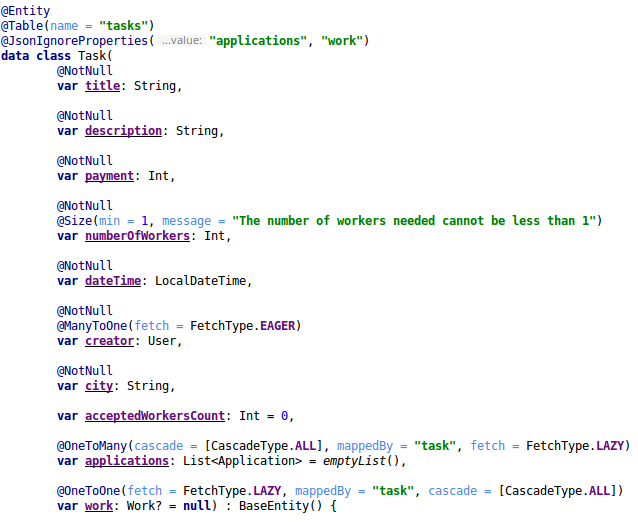
\includegraphics[width=1\textwidth]{images/task_entity.png}}%
            \caption{}
            \label{fig:task_entity}
        \end{figure}
        
        Полетата в Task модела са следните:
        \begin{itemize}
            \item Title - името на обявата.
            \item Description - описание на работата, която ще се извършва.
            \item Payment - сумата, която всеки работник ще бъде заплатен.
            \item NumberOfWorkers - Броя работници, които са нужни за работата.
            \item DateTime - Времето, когато работата ще се извършва.
            \item Creator - Идентификационния номер на създателя на обявата.
            \item City - Градът, в който ще се извършва работата.
            \item AcceptedWorkersCount - Броя работници, които вече са приети за работата.
        \end{itemize}
        
        \newpage
        
         \subsubsection{Application модел}
        
        Application представлява заявление за участие на работа. При желание работник да участва в определена работа, той трябва да създаде заявление. Работодателят има достъп до тези заявления, чрез които преценява кои са най-подходящите работници за неговата работа.
        
        Новото в този модел, показан на фигура \ref{fig:application_entity}, е полето ``uniqueConstraints'' в анотацията ``Table''. Всеки Application има информация за обявата, на която принадлежи и работника, който я е създал. Искаме да не може един работник да създава повече от едно заявление за една и съща работа. Именно за това служи полето ``uniquerContraints'' в анотацията ``Table''. ``UniqueContraints'' очаква списък от полета в таблицата, които не могат да бъдат повтаряни. В този случай желаем да не се повтарят ``user\textunderscore id'' и ``task\textunderscore id''. Тъй като сме обявили полетата в модела от тип ``ManyToOne'' Spring Data автоматично ще ги запише като конкатинира ``\textunderscore id'' към името на полето.
        При опит за повтаряне на двойката полета приложението връща HTTP 400.
        
        \begin{figure}[h]
            \centering
             \makebox[\textwidth][c]{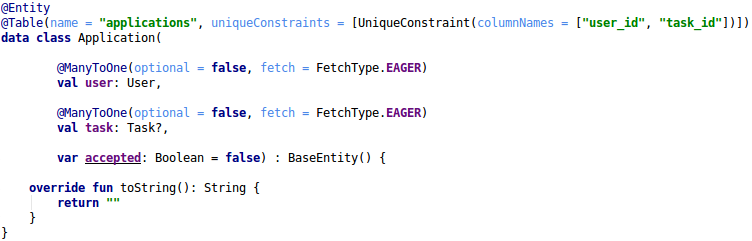
\includegraphics[width=1\textwidth]{images/application_entity.png}}%
            \caption{}
            \label{fig:application_entity}
        \end{figure}
        
        \subsubsection{Work модел}
        
        Новото в Work модела е анотацията \textbf{Enumerated}, на която стойност е \textbf{EnumType.STRING}. Тази анотация служи за да можем да изберем по какъв начин да се запазва ENUM стойността. Това поле показва какъв е статус на работата.
        
        Възможните статуси са:
        \begin{itemize}
            \item IN\textunderscore PROGRESS
            \item ENDED
        \end{itemize}
        
        Ако изберем EnumType.STRING, стойността ще бъде запазена като String. Ако изберем EnumType.ORDINAL, стойността ще бъде запазена като число, обозначаващо позицията на стойността в Enum класа.
        
        \begin{figure}[h]
            \centering
            \makebox[\textwidth][c]{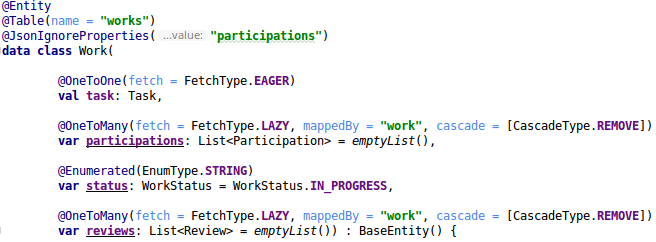
\includegraphics[width=1\textwidth]{images/work_entity.png}}%
            \caption{}
            \label{fig:work_entity}
        \end{figure}
        
        Останалите модели са структурирани на същия принцип.

    \subsection{Основна функционалност}
    Основната функционалност е създадена чрез модела MVC(Model-View-Controller) на Spring. MVC е архитектурен шаблон за дизайн в програмирането, основан на разделянето на бизнес логиката от графичния интерфейс и данните в дадено приложение. В конкретния случай, тъй като няма графичен интерфейс в проекта, не е използванa View частта от шаблона. 
    
    Клиентът контактува единствнео с контролер, който отговаря за работенето с модела, който от своя страна прави промени или извлича данни от базата данни спрямо бизнес логика.

        \subsubsection{Контролери}
        Контролерът е един вид диригента на цялата система. Той определя кои функции трябва да бъдат изпълнени от модела, когато клиент направя заявка към приложението. Контролерът съдържа информация за всички крайни точки, които са достъпни до клиента. 
        
        \begin{figure}[h]
            \centering
            \makebox[\textwidth][c]{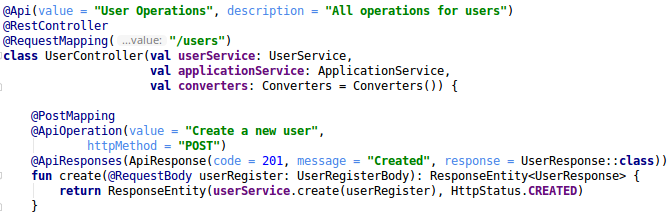
\includegraphics[width=1\textwidth]{images/user_controller.png}}%
            \caption{}
            \label{fig:user_controller}
        \end{figure}
        
        На фигура \ref{fig:user_controller} е показан контролера за потребители и един метод от него. В Spring MVC за да дефинираме клас като контролер го анотираме с анотацията @RestController (Или @Controller ако API-то няма да е RESTful). Анотирайки го казваме на Spring, че този клас ще бъде Компонент, който трябва да бъде регистриран и този Компонент ще служи работата на контролер. Важно е всеки клас, който желаем да използваме като Компонент да бъде анотиран с един от следните анотации:
        \begin{itemize}
            \item Controller(RestController)
            \item Service
            \item Repository
            \item Component
        \end{itemize}
        
        Всеки един от тези анотации има за основа анотацията \textbf{Component}. Анотирайки го с \textbf{Component} казваме на Spring, че желаем да бъде създаден Bean от този тип клас. Създаването на Bean е за да можем да се възползваме от DI(Dependency Injection) и IoC(Inversion of Control), които бяха коментирани в глава 2.
        
        Анотирайки контролера с \textbf{RequestMapping} описваме линк, на който крайните точки на този контролер ще бъдат достъпни.
        
         Метода ``create'' е анотиран с \textbf{PostMapping} за да дефинираме, че този метод може да бъде достъпен чрез POST заявка. На анотацията не е подадена стойност, следователно ако направим POST заявка на URL ``/users'' ще извикаме този метод. 
        
        \textbf{Анотациите започващи с името ``Api'' ще бъдат коментирани по-късно в главата}
        
        В проекта има 5 контролера:
        \begin{itemize}
            \item UserController
            \item TaskController
            \item ApplicationController
            \item WorkController
            \item ReviewController
        \end{itemize}
        
        В аргументите поставяме обект, който очакваме. Spring MVC автоматично десериализира изпратения JSON в обекта, който сме поставили като аргумент. В този случай метода във фиугра \ref{fig:user_controller} очаква обект от типа UseBody. Всеки POST метод в контролер очаква Body клас, който представлява абстракция на JSON-а, който се очаква. В този случай очакваме JSON с полета:
        \begin{itemize}
            \item firstName
            \item lastName
            \item email
            \item password
            \item dateOfBirth
            \item phoneNum
        \end{itemize}
        
        За да кажем, че обекта който е в аргументите го очакваме като JSON в тялото на заявката го анотираме с анотацията \textbf{RequestBody}.
        
        При изпращане на заявка без такъв JSON или с грешен такъв се връща HTTP 400 Bad Request.
        
        Всеки метод в контролера връща обект от тип \textbf{ResponseEntity}. Обекта позволява за пълен контрол върху HTTP отговора. В него дефинираме тялото на отговора като първи параметър и HTTP статуса, който се връща като втори.
        
        За създаването на тялото на HTTP отговора контролера извиква конкретен метод от услуга, който извършва всичката бизнес логика и мнаипулира данните в базата данни.
        
        Това, което всъщност се връща е обект от типа UserResponse. Тъй като искаме да имаме контрол върху това, което връщаме на потребителя искаме да имаме специални класове, които действат като отговор на заявките.
        Повечето от моделите имат съответен Response клас.
        На фигура \ref{fig:user_response} е показан Response класа на потребител.
        Тъй като паролата е чувствителна информация, не желаем да я връщаме като отговор на заявка.
        
        \begin{figure}[h]
            \centering
            \makebox[\textwidth][c]{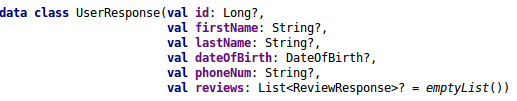
\includegraphics[width=1\textwidth]{images/user_response.png}}%
            \caption{}
            \label{fig:user_response}
        \end{figure}
        
        Услугата, която ползваме сме сложили в конструктура на класа и в този случай услугата се казва ``UserService''. Spring автоматично ще намери Bean-а и ще го инжектира в класа.
        
        \subsubsection{Услуги}
        Услугите са Model частта от MVC шаблона. Те изпълняват всичката бизнес логика, когато клиент направи заявка към приложението. Не желаем услугата да има каквото и да било знание за контролера, който го извиква. Една то целите на MVC шаблона е всеки компонент да бъде колкото се може по-отделен от останалите компоненти. Това помага не само за по-доброто преизползване и дебъгване на приложението, но и по-лесното писане на тестове върху конкретния компонент. Всеки контролер има съответен клас от типа ``услуга''.
        На фигура \ref{fig:user_service} е показан класа UserService заедно с метода \textbf{create} от него.
        
        \begin{figure}[h]
            \centering
            \makebox[\textwidth][c]{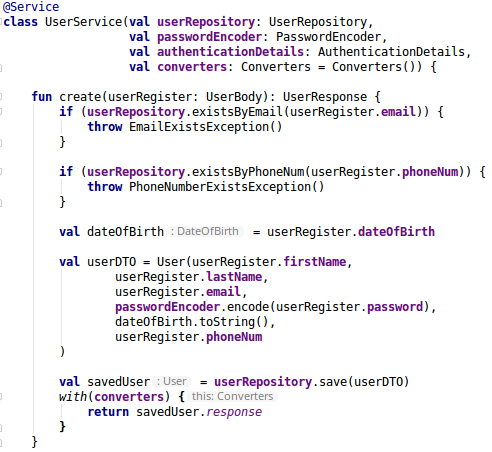
\includegraphics[width=1\textwidth]{images/user_service.png}}%
            \caption{}
            \label{fig:user_service}
        \end{figure}
        
        В конструктура на класа се очаква да се подадат четири обекта:
        \begin{itemize}
            \item UserRepository - класа, който представлява австракция за манипулиране на базата данни (Повече информация по-надолу в главата)
            \item PasswordEncoder - обект за кодиране на парола на потребител. Никога не искаме да пазим паролата на потребител в чист вид. 
            \item AuthenticationDetails - Клас, създаден от мен, за лесното извличане  на имейла на потребителя, който прави заявката.
            \item Converters - Клас, който съдържа удължителни функции за превръщане на клас от тип Entity в тип Response.
        \end{itemize}
        
        Spring авотматично ще ни ги осигури при стартиране на приложението.
        
        \begin{figure}[h]
            \centering
            \makebox[\textwidth][c]{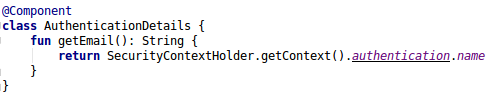
\includegraphics[width=1\textwidth]{images/auth_details.png}}%
            \caption{}
            \label{fig:auth_details}
        \end{figure}
        
        На фигура \ref{fig:auth_details} е показан класа \textbf{AuthenticationDetails}. В него има един метод на име \textbf{SecurityContextHolder}, който ни предоставя имейла, подаден при аутентикацията. Причината да се нуждаем от този клас е за да можем да получим повече информация за потребителя, който прави заявката, когато имаме нужда от това.
        
        \begin{figure}[h]
            \centering
            \makebox[\textwidth][c]{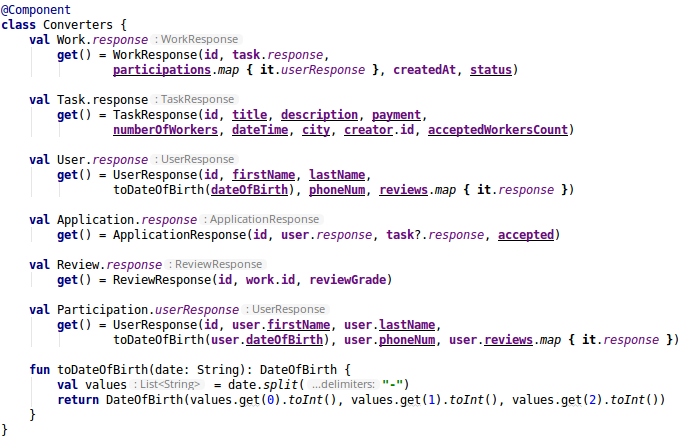
\includegraphics[width=1\textwidth]{images/converters}}%
            \caption{}
            \label{fig:converters}
        \end{figure}
        
        \textbf{Converters}, показан във фигура \ref{fig:converters} е класа, който съдържа всички удължителни функции за Entity класовете за превръщане в Response класове.  При промяна на Response клас единствено трябва да се промени удължаващата функция в този клас. Тъй като тези методи се използват на множествно места искаме дефиницията на превръщането от Entity в Response да бъде централизирано. Ако променим нещо по Response клас трябва да актуализираме единствено в Converters класа.
        
        
        \subsubsection{Хранилище}
        Хранилищата са интерфейси, предоставени от Spring Data JPA, за манипулиране и извличане на данните от PostgreSQL базата. За всяка таблица искаме да имаме по едно хранилище, което ще се грижи за действията по нея. Ще разберем как работят те като разгледаме UserRepository на фигура \ref{fig:user_repository}.
        
        Създавайки интерфейс, който наследява \textbf{JpaRepository}, Spring автоматично ни позволява да използваме вече дефинирани методи. Част от тях са:
        \begin{itemize}
            \item save - запозва подадения обект от тип User в таблицата
            \item findById - намира ред от таблицата спрямо Id-то, което сме му подали и ни го връща като обект от тип \textbf{Optional<User>}
            \item deleteById - изтрива ред в таблицата спрямо подаденото Id
        \end{itemize}
        
        \begin{figure}[h]
            \centering
            \makebox[\textwidth][c]{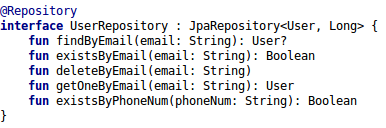
\includegraphics[width=1\textwidth]{images/user_repository.png}}%
            \caption{}
            \label{fig:user_repository}
        \end{figure}
        
        Интерфейсът, който наследяваме трябва да получи типа на обектите, които ще бъдат запазени в базата данни и типа на Id-то, което те ще имат. В нашия случай желаем да запазваме User обекти, на които Id-то ще бъде от тип Long.
        
        Често обаче имаме нужда от по-специфични методи за манипулиране на данните. В този случай имаме нужда от метод, който връща Потребител спрямо неговият имейл адрес. Spring предоставя възможността да изграждааме такива методи единствено чрез името, което слагаме на метода. 
        В класа е създаден един метод на име findByEmail. Спрямо името на метода Spring автоматично разбира каква е нашата цел. В документацията на Spring Data JPA \parencite{Repository} може да се намери повече информация.
        
        Добавените от нас методи са:
        \begin{itemize}
            \item findByEmail
             Връща потребител спрямо неговият имейл адрес.
            \item existsByEmail 
            Връща boolean стойност спрямо това дали съществува потребител с подадения имейл адрес
            \item deleteByEmail
            Премахва потребител от таблицата спрямо неговия имейл адрес
            \item getOneByEmail - намира потребител от таблицата спрямо неговия имейл адрес. Разликата между \textbf{getOneByEmail} и \textbf{findByEmail} е начинът, по който данните се извличат от базата. FindByEmail извлича потребител \textbf{EAGERLY}, докато getOneByEmail го извлича \textbf{LAZILY}.
            \item existsByPhoneNum
            Връща boolean спрямо това дали потребител с подадения телефонен номер съществува.
        \end{itemize}
        
        Останалите хранилища са направени по същия модел.
        
        Едно от изискванията, които имаме към приложението е да може да се филтрира спрямо полетата на Task. За да изпълним това изискване трябва да се възползваме от QueryBuilder предоставен от Spring Data. 
        
        \begin{figure}[h]
            \centering
            \makebox[\textwidth][c]{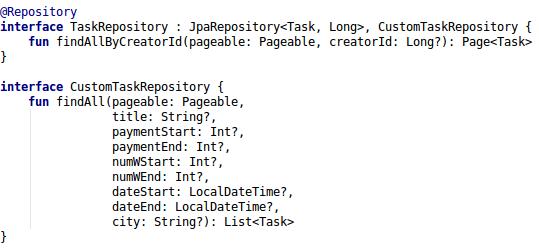
\includegraphics[width=1\textwidth]{images/task_repository.png}}%
            \caption{}
            \label{fig:task_repository}
        \end{figure}
        
        За тази цел трябва да добавим нов метод, на който искаме да добавим тяло. Започваме със създаването на \textbf{interface}, който дефинира метод с всичките полета в един Task, както е показано на фигура \ref{fig:task_repository}. След това, за да може \textbf{TaskRepository} да използва метода искаме да наследява създадения от нас interface.
        Последната стъпка е да създадем клас, който да наследява създадения от нас interface и да попълним метода.
        
        \begin{figure}[h]
            \centering
            \makebox[\textwidth][c]{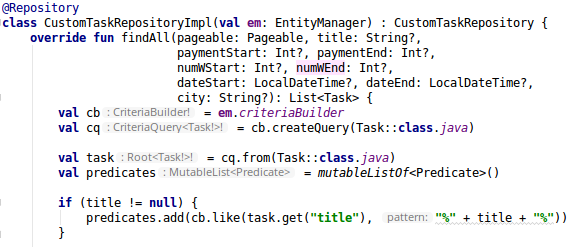
\includegraphics[width=1\textwidth]{images/custom_task_repository.png}}%
            \caption{}
            \label{fig:custom_task_repository}
        \end{figure}
        
        На фигура \ref{fig:custom_task_repository} е показана имплементацията на създадения от нас клас. Методът приема полетата на един Task и спрямо това дали са null ги добавя в списък от \textbf{Predicate}. За да създадем персонализирания query искаме първо да използваме предоставения от Spring \textbf{EntityManager}. Той е централния обект, който комуникира с базата данни и чрез него извличаме обект от тип \textbf{CriteriaBuilder}. Така съставяме Query, на което подаваме резултатния клас (в този случай Task) и класа спрямо който ще извършваме Query-то(отново Task). След като всичките нужни предикати са добавени ги добавяме към Query-то(cq) и го изпълняваме.
        Резултатния списък е всички Task-ове, които отговарят на филтъра.
        
        Причината да извличаме данните чрез QueryBuilder е поради натоварване. Възможно е първо да се извлиекат всички Task-ове от базата данни и след това да се филтрира спрямо полетата, но в случая, че имаме голям брой Task-ове тяхното извличане би било бавен и тежък процес.
        
        \subsubsection{Swagger}
        За имплементирането на Swagger е нужно създаването на един \textbf{Configuration} клас.
        
        \begin{figure}[h]
            \centering
            \makebox[\textwidth][c]{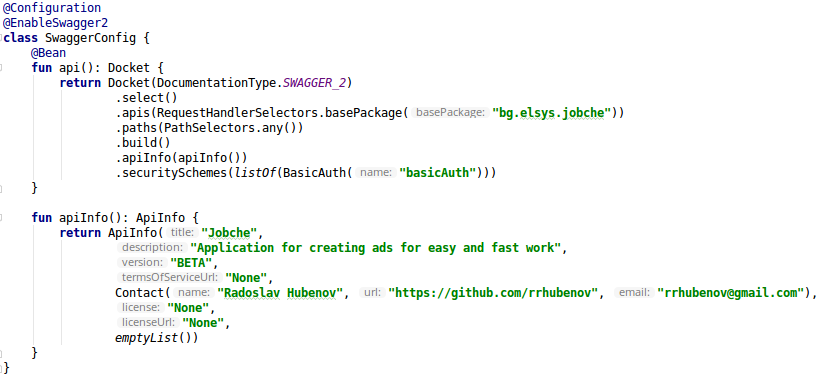
\includegraphics[width=1\textwidth]{images/swagger_config.png}}%
            \caption{}
            \label{fig:swagger_config}
        \end{figure}
        
        Този клас е показан на фигура \ref{fig:swagger_config}. Анотираме класа с \textbf{Configuration} и \textbf{EnableSwagger2}. Както е показано трябва да добавим един метод, който връща Bean от тип \textbf{Docket}. Причината за това е, че Swagger има нужда от конфигурации, които да настроим. Като например в кой пакет се намират контролерите. В този случай сме посочили основния пакет на приложението ``bg.elsys.jobche''. Swagger автоматично ще намери всички класове анотирани със Spring анотация Controller и ще ги добави към документацията. 
        
        В много случаи обаче желаем да добавим повече информация за конкретната крайна точка. Това се случва чрез анотации започващи с \textbf{Api}. Както показахме на фигура \ref{fig:user_controller} чрез тях можем да добавим наши обяснения към документацията. Като пример функцията на специфичната крайна точка, какво връща, какво очаква и тн.
    
\section{Тестова част}

    Много важна част от създаването на проекта са тестовете. Старал съм се да спазвам TDD(Test Driven Development) принципи при създаването му. TDD - изработка чрез тестове, спрямо дефиницията в уикипедия, е метод за разработка на софтуер, при който се спазва следният работен цикъл: първо се пишат тестови варианти (test cases), които да покрият изискванията за новия изходен код, а чак след това се пише програмния код така, че да покрива тези тестове. Кент Бек, който се счита за създател на този метод, заявява през 2003, че TDD цели един опростен дизайн\parencite{TDD}. 
    
    За спазване и разработка чрез TDD съм използвал презентацията на Uncle Bob\parencite{KotlinTDD}.
    В него той дефинира три правила за използването на TDD:
    \begin{enumerate}
        \item Не се пише фунцкионален код, освен ако е с цел да се накара тест да мине.
        \item Пишеш само толкова тестов код, колкото е нужно за да се провали.
        \item Пише се единствено толкова функционален код, колкото е необходимо за да мине теста.
    \end{enumerate}
    
    Тези три правила те вкарват в един цикъл на изработване на тестове и писане на функционален код. Пише се част от тест, пише се част от функционалната част. Предимствата на TDD са особено подходящи за нови програмисти. Използвайки тази методология програмиста успява да си представи архитектурата на проекта, който иска да създаде. Кара го да мисли за това какво функционалния код трябва да прави, отколкото \textbf{КАК} да го прави. Въпреки това писането на тестове не е лесна работа. През целия проект писането на тестове отне 80 процента от цялото време. Средно за всеки ред функционален код е написан 2 реда тестове. Те също имат архитектура, която трябва да се спазва и поради тази причина писането им не бе лесна задачка.
    
    \subsection{Unit тестове}
    Unit тест представлява тест върху един компонент. Компонент в този случай е клас. В проекта за всеки контролер и всяка услуга има по един Unit Test клас, който тества всичките методи и изпълнява test cases. Както се споменава в глава 2 за писането на тестове е използван JUnit5, mockK и assertJ.
    
        \subsubsection{Тестове върху контролери}
        При писане нa Unit тестове желаем да тестваме отделните компоненти изцяло отделени от останалите или от зависимостите си. В контекста на UserController искаме да бъде тестван без да се притесняваме дали UserService, или която и да е друга зависимост, работят правилно. Тестът трябва да бъде изцяло съсредоточен върху методите и функционалността единствено на компонента, който тестваме.
        
        \begin{figure}[h]
            \centering
            \makebox[\textwidth][c]{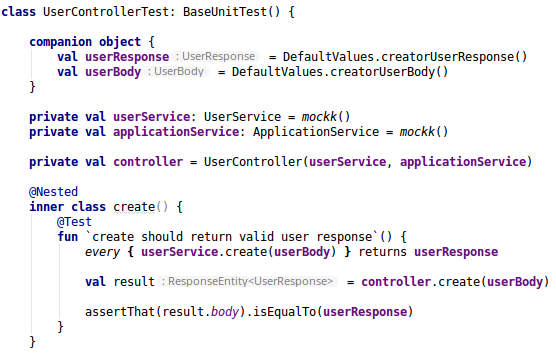
\includegraphics[width=1\textwidth]{images/user_controller_test.png}}%
            \caption{}
            \label{fig:user_controller_test}
        \end{figure}
        
        На фигура \ref{fig:user_controller_test} е показан класа \textbf{UserControllerTest} и един тестов метод от него. Всеки UnitTest наследява класа \textbf{BaseUnitTest}, който осигурява анотацията \textbf{@ExtendWith(MockKExtension::class)}. Това е нужно за да бъде регистриран MockK като осигурител на Мок обектите. Мок обектите служат като заместител на зависимостите, които някой клас използва. В този случай мокваме двете услуги, които UserController класа иползва - UserService и ApplicationService. След като са мокнати, за да няма грешка в тестове, трябва
        да контролираме какво се случва при изпълнението на техните методи. За това служи и метода \textbf{every}. Казваме му при изпълнението на метода create с подаден аргумент userBody върни обект userResponse. По този начин осигуряваме, че независимо дали зависимостите работят правилно или грешно, единствено тестваме метода от компонента дали се изпълнява правилно.
        
        \subsubsection{Тестове върху услуги}
        Тестовете на услугите се извършват по същия принцип като тестовете на контролерите. Мокваме зависимостите на класа и очакваме, че той ще върне отоговра, който очакваме.
        
    
    \subsection{Integration тестове}
    Integration тестовете служат за тестване на цялостен процес на софтуера. Симулира се цялостна заявка към бекенда, и се очаква че ще се върне отговора, който очакваме.
    
    \begin{figure}[h]
            \centering
            \makebox[\textwidth][c]{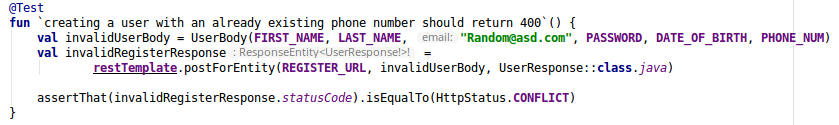
\includegraphics[width=1\textwidth]{images/user_int_test.png}}%
            \caption{}
            \label{fig:user_int_test}
        \end{figure}
        
    На фигура \ref{fig:user_int_test} е показан един тест от UserIntegrationTest класа. Важно е името на метода да обозначава колкото се може по-ясно каква е целта на теста. Поради тази причина използваме функционалността на Kotlin за именуване с празно място между думите чрез обграждане със знака \textbf{`}. В теста при опит за създаване на потребител, чийто телефонен номер вече регистриран отговора да е от тип HTTP 400. За създаване на заявката използваме обект от тип TestRestTemplate. Той ни позволява да изпълняваме различен тип заявки към дефиниран линк и да получим обратно отговор като му предоставяме в какъв обект да десериализира JSON отговора.
    В този случай единствено искаме да знаем, че статус кода, който е върнат е 400.
    